\chapter{Kết quả thực nghiệm}
Chương này trình bày các tiêu chí đánh giá, quá trình hiện thực các thực nghiệm cho mô hình đề xuất và giải thuật HOTSAX, cũng như phân tích kết quả thực nghiệm đạt được.
Môi trường thực nghiệm:
\begin{itemize}
\item Hệ điều hành: MacOS Big Sur version 11.3
\item Ngôn ngữ: Python3
\item Framework: Keras 2.3.1 với nhân là Tensorflow và các thư viện như: numpy, pandas, sklearn…
\item Cấu hình máy tính: Macbook Pro 2020 - MWP42; 2.0 GHz Quad-Core Intel Core i5 gen-10th; RAM: 16 GB.
\end{itemize}

\section{Tiêu chí đánh giá}



Để đánh giá kết quả của phương pháp đề xuất với các phương pháp khác, chúng tôi sẽ hiện thực giải thuật HOT SAX để làm cơ sở so sánh. 

Đối với bài toán dự báo, kết quả dự báo của mô hình sẽ được đo và so sánh dựa trên độ đo \textbf{Mean Square Error (MSE)} và \textbf{Mean Absolute Error (MAE)}.

\textbf{Mean Squared Error:} cũng là một độ đo mức độ sai lệch của dự báo, nhưng mức độ sai lệch sẽ được tính bằng trung bình tổng bình phương độ sai lệch của dự báo và thực tế.

\begin{equation}
\label{eq:24}
MSE =\frac{1}{n}\sum_{i=1}^{n}(y_i-\varphi_i)^2
\tag{24}
\end{equation}

\textbf{Mean Absolute Error:} Là độ đo mức độ sai lệch của dự báo mà không xem xét tới hướng của chúng. Được tính trung bình sự khác biệt tuyệt đối giữa giá trị dự báo và giá trị quan sát thực tế của các mẫu thử nghiệm trong đó tất cả các khác biệt có trọng số bằng nhau.

\begin{equation}
\label{eq:25}
MAE =\frac{1}{n}\sum_{i=1}^{n}|y_i-\varphi_i|
\tag{25}
\end{equation}

Đối với \textbf{MSE}, việc bình phương trọng số trước khi tính trung bình, làm cho sự sai biệt giữa giá trị dự báo và thực tế tăng lên, giúp cho độ đo này có trọng số lớn với nhưng sai lệch lớn, tức là chỉ một vài giá trị dự báo sai lệch lớn so với giá trị thực tế cũng có thể làm cho giá trị \textbf{MSE} lớn mặc dù những giá trị khác được dự báo chính xác. Tuy nhiên, độ đo \textbf{MSE} trong nhiều trường hợp có thể lớn mà không nói lên được ý nghĩa của mô hình là tốt hay xấu. Mặt khác, độ đo này phụ thuộc vào độ lớn của tập dữ liệu, vì nó dựa trên giá trị dự báo và giá trị thực tế. vì thế, đối với dữ liệu có biên độ lớn thì độ lỗi của mô hình sẽ rất lớn so với mô hình dự báo cho dữ liệu có biên độ nhỏ hơn.

Sai số \textbf{MAE} được tính bằng trung bình trị tuyệt đối sai số dự báo của mô hình đề xuất, và các giá trị thu được của độ đo này sẽ được mô hình hoá bằng cách sử dụng phân phối Gauss. Trên tập dữ liệu kiểm thử 2 $V_{A}$, giá trị logPD của lỗi dự báo sẽ được tính toán và dùng làm giá trị phát hiện bất thường. Một giá trị \textit{ngưỡng} (threshold) sẽ được chọn,  sao cho các giá trị logPD của các điễm dữ liệu bất thường sẽ nhỏ hơn giá trị ngưỡng này, và các giá trị logPD của các điểm dữ liệu bình thường sẽ có giá trị lớn hơn giá trị ngưỡng này. Để từ đó, đối với dữ liệu trên tập kiểm tra \textit{T}, chúng tôi sử dụng giá trị ngưỡng để phát hiện bất thường. Với các điểm dữ liệu có giá trị logPD lớn hơn giá trị ngưỡng, chúng tôi sẽ xem đó là dữ liệu bình thường. Và các điểm dữ liệu có giá trị logPD nhỏ hơn giá trị ngưỡng, chúng tôi sẽ xem đó là dữ liệu bất thường.

Trong một vài thử nghiệm, chúng tôi đã cân nhắc giữa tối ưu sai số \textbf{MAE}, \textbf{MSE} cho mô hình và kết quả phát hiện bất thường. Nếu chọn tối ưu mô hình cho dự báo bằng cách giảm sai số dự báo, đây không phải là cách tốt nhất để phát hiện bất thường. Sai số dự báo thấp trên tập kiểm thử 2 $V_{A}$ và tập kiểm tra \textit{T} sẽ gây khó khăn trong việc tìm giá trị ngưỡng để tách biệt dữ liệu bình thường và dữ liệu bất thường, có thể gây ra nhiều cảnh báo sai.

Đối với bài toán phát hiện chuỗi con bất thường, kết quả phát hiện chuỗi con bất thường sẽ được so sánh với các chuỗi con bất thường đã được đánh dấu từ các nhà nghiên cứu đi trước. Tuỳ thuộc vào bộ dữ liệu, có những bộ dữ liệu được đánh dấu nhiều chuỗi con bất thường, cũng có những bộ dữ liệu chỉ được đánh dấu một chuỗi con bất thường. Để thuận tiện trong việc so sánh giữa mô hình đề xuất và giải thuật HOTSAX, chúng tối quyết định chỉ phát hiện chuỗi con bất thường bậc 1 trong mỗi bộ dữ liệu, tức là chuỗi con bất thường có sự khác biệt lớn nhất so với phần còn lại của bộ dữ liệu. Do đó, giải thuật HOTSAX sẽ được thiết lập để tìm ra chuỗi con bất thường bậc 1, và chúng tôi kỳ vọng mô hình đề xuất cũng phát hiện ra chuỗi con bất thường này. Sau đó, chúng tôi sẽ tiến hành so sánh kết quả phát hiện bất thường của cả hai phương pháp. Đây là cách đánh giá hiệu quả của phát hiện chuỗi con bất thường trên dữ liệu chuỗi thời gian thường được cộng đồng nghiên cứu lĩnh vực này sử dụng.

Một phần không thể thiếu, đó là thời gian thực thi của mô hình đề xuất và giải thuật HOTSAX. Mặc dù hai phương pháp với hai hướng tiếp cận và hai phương thức hoạt động khác nhau, nhưng đây cũng sẽ là một thông số để tham khảo trong việc so sánh giữa hai phương pháp này. Đối với HOTSAX, thời gian thực thi chỉ là thời gian chạy giải thuật HOTSAX trên bộ dữ liệu. Đối với mô hình đề xuất, thời gian thực thi là tổng hợp thời gian của các bước, bao gồm: tiền xử lý dữ liệu, huấn luyện mô hình, dự báo dữ liệu, phát hiện bất thường. Trong đó, thời gian cho bước huấn luyện mô hình sẽ chiếm phần lớn thời gian thực thi của mô hình đề xuất. Để đảm bảo cho việc đo đạc thời gian được chính xác nhất, chúng tôi lần lượt thực hiện đo thời gian thực thi của hai phương pháp trên 08 bộ dữ liệu trong vòng 100 lần. Sau đó, kết quả thu được sẽ lấy trung bình để cho ra thời gian thực thi của từng phương pháp trên từng bộ dữ liệu.

\section{Thực nghiệm}
\subsection{Giải thuật HOTSAX}
\begin{figure}[H]
    \centering
    
\includegraphics[scale=0.75]{./content/images/5-1.png}
    \caption{Mô hình giải thuật HOT SAX}
    \label{fig:5-1}
\end{figure}

Như đã được trình bày, dữ liệu ban đầu sẽ được chuẩn hóa thành chuỗi thời gian mới có trung bình bằng 0 và độ lệch chuẩn bằng 1 (Chuẩn hóa z-score). Chuỗi dữ liệu sau khi được chuẩn hóa sẽ được thu giảm số chiều bằng phương pháp PAA. Chuỗi dữ liệu sau khi được thu giảm sẽ được rời rạc hóa bằng phương pháp SAX. Sau cùng, giải thuật HOT SAX sẽ được sử dụng để nhận diện đoạn bất thường.

Các thông số của giải thuật, tuỳ thuộc vào bộ dữ liệu mà ta có thông số khác nhau, bảng \ref{tab:5-1}:
\begin{itemize}
\item Bề rộng cửa sổ trượt \textit{n}.
\item Hệ số thu giảm số chiều \textit{w} trong phương pháp PAA.
\item Số lượng các kí tự rời rạc hóa \textit{a} trong phương pháp SAX.
\end{itemize}

\subsection{Mô hình đề xuất}
\begin{figure}[H]
    \centering
    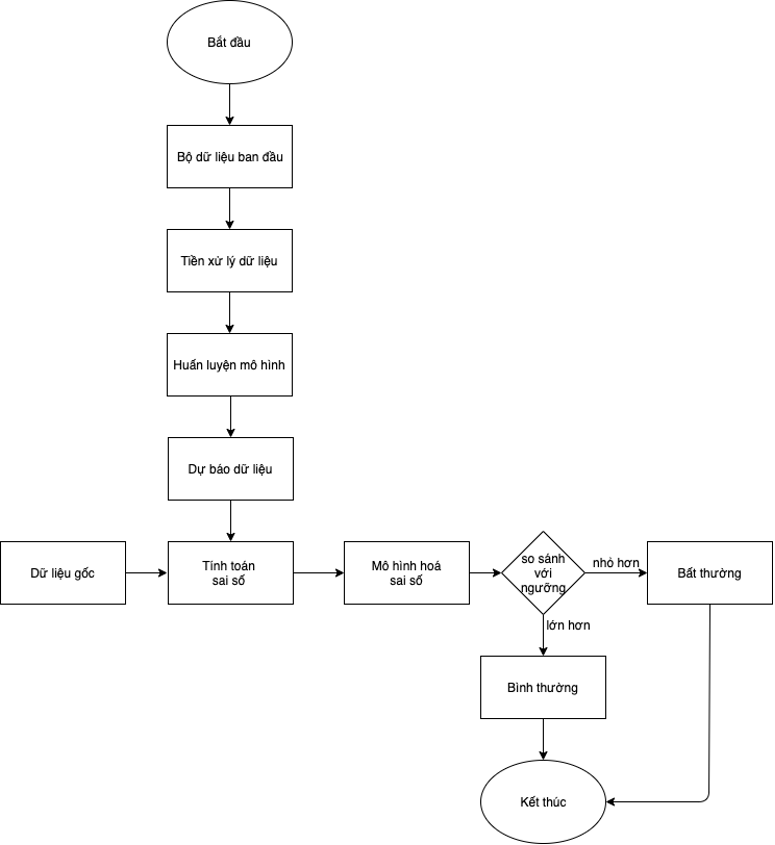
\includegraphics[scale=1.25]{./content/images/5-2.png}
    \caption{Mô hình đề xuất}
    \label{fig:5-2}
\end{figure}

Trong thực nghiệm, chúng tôi tiến hành huấn luyện mô hình, dự báo dữ liệu và phát hiện bất thường trên từng bộ dữ liệu, hình \ref{fig:5-2}. Đối với mỗi bộ dữ liệu, các điểm dữ liệu bất thường được chia thành các tập $V_{A}$ và \textit{T}. Các tập này sau đó được tăng cường với các điểm dữ liệu bình thường. Dữ liệu còn lại được chia thành các tập dữ liệu \textit{N} và $V_{N}$ cho quá trình huấn luyện mô hình. Các bộ dữ liệu có chu kỳ lặp lại được chia theo cách mà các chu kỳ vẫn được nguyên vẹn. Chúng tôi cũng tiến hành chuẩn hóa dữ liệu. Giá trị trung bình và độ lệch chuẩn của tập huấn luyện được sử dụng để chuẩn hóa các tập dữ liệu khác. Cuối cùng, mỗi tập dữ liệu sẽ được chuyển đổi thành định dạng theo yêu cầu của thuật toán. Vì vậy, mỗi mẫu dữ liệu đầu vào sẽ bao gồm số bước như đã thiết lập ở \textit{lookback}, và đầu ra sẽ bao gồm số bước như đã thiết lập ở \textit{lookahead}. Từ dữ liệu mới được dự báo, chúng tôi tiến hành tính toán và mô hình hoá sai số cho bước phát hiện bất thường. Chi tiết kiến trúc của các mô hình thực nghiệm như trong Bảng \ref{tab:5-1}.

% \usepackage{graphicx}


\begin{table}[H]
\centering
\resizebox{\linewidth}{!}{%
\begin{tabular}{|l|l|l|l|l|l|} 
\hline
\textbf{Bộ dữ liệu} & \textbf{HOTSAX}                                                             & \textbf{Kiến trúc mô hình}                                                                                                                  & \textbf{Adam Optimizer}                                                   & \begin{tabular}[c]{@{}l@{}}\textbf{Lookback,}\\\textbf{Lookahead}\end{tabular} & \textbf{Batch size}  \\ 
\hline
ECG                 & \begin{tabular}[c]{@{}l@{}}n: 128\\w: 8\\a: 3\end{tabular}                  & \begin{tabular}[c]{@{}l@{}}Recurrent: \{60\} \\Dropout: 0.1 \\Recurrent: \{30\} \\Dropout: 0.1 \\Dense: \{1\} \\Linear Activation\end{tabular} & \begin{tabular}[c]{@{}l@{}}Learning Rate: 0.1 \\Decay: 0.99\end{tabular}  & 8,5                                                                            & 1024                 \\ 
\hline
nhiệt độ máy Numenta & \begin{tabular}[c]{@{}l@{}}n: 128\\w: 8\\a: 3\end{tabular}                  & \begin{tabular}[c]{@{}l@{}}Recurrent: \{80\} \\Dropout: 0.1 \\Recurrent: \{20\} \\Dropout: 0.1 \\Dense: \{1\}\\Linear Activation\end{tabular}  & \begin{tabular}[c]{@{}l@{}}Learning Rate: 0.05 \\Decay: 0.99\end{tabular} & 24,12                                                                          & 256                  \\ 
\hline
power\_data         & \begin{tabular}[c]{@{}l@{}}n: 1000\\ w: 8\\ a: 3\end{tabular}               & \begin{tabular}[c]{@{}l@{}}Recurrent: \{300\} \\Dropout: 0.2 \\Dense: \{1\}\\Linear Activation\end{tabular}                                   & \begin{tabular}[c]{@{}l@{}}Learning Rate: 0.01 \\Decay: 0.99\end{tabular} & 1,1                                                                            & 672                  \\ 
\hline
TEK16               & \begin{tabular}[c]{@{}l@{}}n: 128\\w: 8\\a: 3\end{tabular} & \begin{tabular}[c]{@{}l@{}}Recurrent: \{80\} \\Dropout: 0.2 \\Recurrent: \{30\} \\Dropout: 0.2 \\Dense: \{1\}\\Linear Activation\end{tabular}  & \begin{tabular}[c]{@{}l@{}}Learning Rate: 0.01 \\Decay: 0.99\end{tabular} & 1,1                                                                            & 1000                 \\ 
\hline
stock\_20\_0        & \begin{tabular}[c]{@{}l@{}}n: 128\\w: 8\\a: 3\end{tabular}                  & \begin{tabular}[c]{@{}l@{}}Recurrent: \{60\} \\Dropout: 0.1 \\Recurrent: \{30\} \\Dropout: 0.1 \\Dense: \{1\}\\Linear Activation\end{tabular}  & \begin{tabular}[c]{@{}l@{}}Learning Rate: 0.1 \\Decay: 0.99\end{tabular}  & 5,3                                                                            & 256                  \\ 
\hline
memory              & \begin{tabular}[c]{@{}l@{}}n: 128\\w: 8\\a: 3\end{tabular}                  & \begin{tabular}[c]{@{}l@{}}Recurrent: \{60\} \\Dropout: 0.1 \\Recurrent: \{30\} \\Dropout: 0.1 \\Dense: \{1\}\\Linear Activation\end{tabular}  & \begin{tabular}[c]{@{}l@{}}Learning Rate: 0.1 \\Decay: 0.99\end{tabular}  & 5,3                                                                            & 256                  \\ 
\hline
ann\_gun\_CentroidA & \begin{tabular}[c]{@{}l@{}}n: 128\\w: 8\\a: 3\end{tabular}                  & \begin{tabular}[c]{@{}l@{}}Recurrent: \{80\} \\Dropout: 0.2 \\Recurrent: \{30\} \\Dropout: 0.2 \\Dense: \{1\}\\Linear Activation\end{tabular}  & \begin{tabular}[c]{@{}l@{}}Learning Rate: 0.01 \\Decay: 0.99\end{tabular} & 1,1                                                                            & 150                  \\
\hline
\end{tabular}
}
\caption{Thông số thiết lập của HOTSAX và mô hình đề xuất}
\label{tab:5-1}
\end{table}

\subsection{Duy trì trạng thái LSTM trong Keras (State Maintenance)}
Keras cung cấp hai cách khác nhau để \textit{duy trì trạng thái} (state maintenance) của LSTM.
\begin{enumerate}
\item \textit{Chế độ mặc định} (Default Mode): Được thiết lập với \textit{stateful} = \textit{false}.\\
Mỗi \textit{mẫu} (sample) trong một \textit{batch} được giả định là độc lập và \textit{trạng thái} (state) chỉ được duy trì qua \textit{các chuỗi đầu vào riêng lẻ} (individual input sequences).
\item \textit{Chế độ duy trì trạng thái} (Stateful Mode): Được thiết lập với \textit{stateful} = \textit{true}.\\
Trong chế độ này, \textit{trạng thái khối} (cell state) được duy trì giữa các \textit{batch} huấn luyện khác nhau. Trạng thái của mẫu thứ \textit{i} trong \textit{batch} hiện tại, sẽ được sử dụng để làm \textit{trạng thái ban đầu} (initial state) cho \textit{mẫu} (sample) thứ \textit{i} của \textit{batch} kế tiếp. Trong một \textit{batch}, \textit{các mẫu riêng lẻ} (individual samples) vẫn độc lập với nhau. Một lỗi thường hay gặp trong chế độ này là việc \textit{trộn dữ liệu} (shuffle data). Để duy trì trạng thái giữa các \textit{batch}, giả định ánh xạ \textit{một-một} giữa các mẫu của các \textit{batch} liên tiếp được sử dụng, và cần tránh trộn dữ liệu trong chế độ này.
\end{enumerate}

Điều này có ý nghĩa đối với các tập dữ liệu có xu hướng lặp lại các chu kỳ. Nó sẽ giúp mô hình của chúng ta dễ dàng học được các xu hướng của dữ liệu, và dự báo chính xác hơn. Trong công tác phát hiện bất thường, điều này thực sự rất quan trọng. 
%\pagebreak

\section{Kết quả thực nghiệm}
\subsection{Bộ dữ liệu điện tâm đồ ECG}
Mạng LSTM xếp chồng được thiết lập với \textit{lookback} là 8, \textit{lookahead} là 5, với hai tầng ẩn lần lượt 60 nốt LSTM và 30 nốt LSTM, theo sau là tầng kết nối đầy đủ với 1 nơ-ron đầu ra, \textit{hệ số học} (dropout) là 0.1. Chúng tôi huấn luyện mô hình với bộ thông số \textit{Adam optimizer}, \textit{learning-rate} là 0.1, \textit{decay} là 0.99, và 600 epoch có điều kiện dừng sớm, \textit{batch-size} là 256. Mặc dù bộ dữ liệu này có chu kỳ, tức là chu kỳ của nhịp tim. Nhưng chúng tôi nhận thấy, không cần phải duy trì trạng thái LSTM qua các \textit{batch} vẫn cho kết quả tốt, nên \textit{stateful} bằng \textit{false}. Giá trị MSE trên tập huấn luyện là 0.0232. Từ tập kiểm thử 2 $V_{A}$, với giá trị ngưỡng bằng -5, tất cả các điểm dữ liệu có giá trị logPD nhỏ hơn giá trị ngưỡng, chúng tôi xác định đó là các điểm bất thường, và ngược lại. Các điểm dữ liệu có giá trị logPD lớn hơn giá trị ngưỡng, chúng tôi xác định đó là các điểm bình thường. Với cách tiếp cận tương tự, chúng tôi dùng giá trị ngưỡng này cho tập kiểm tra \textit{T}.

\begin{figure}[H]
    \centering
    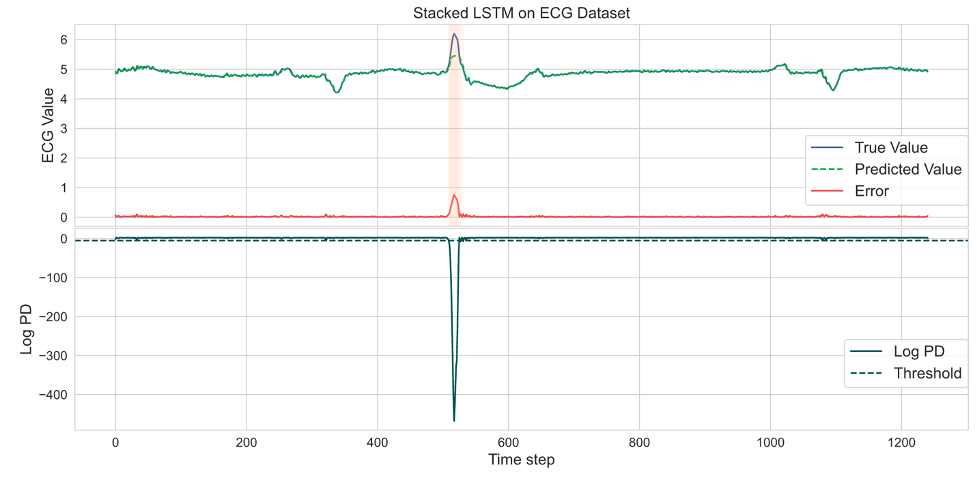
\includegraphics[scale=1]{./content/images/5-7.png}
    \caption{Phát hiện bất thường trên bộ dữ liệu ECG của mô hình đề xuất}
    \label{fig:5-7}
\end{figure}

Đối với giải thuật HOTSAX, chúng tôi vẫn tiến hành thiết lập các thông số như Bảng \ref{tab:5-1}, với bề rộng của sổ trượt \textit{n} là 128, hệ số thu giảm số chiều \textit{w} là 8 và số lượng các ký tự rời rạc hoá \textit{a} là 3. Bộ dữ liệu đã được tiền xử lý để có thể phù hợp với giải thuật HOTSAX từ các chuyên gia trong các công trình nghiên cứu trước đó.

\begin{figure}[H]
    \centering
    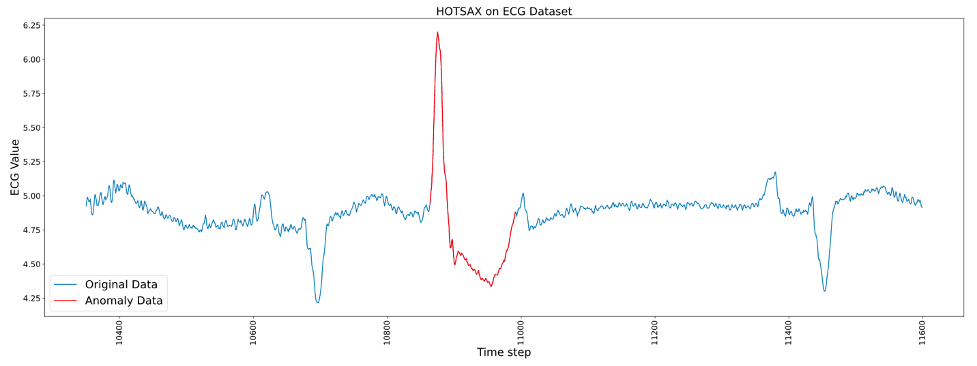
\includegraphics[scale=0.85]{./content/images/5-8.png}
    \caption{Phát hiện bất thường trên bộ dữ liệu ECG của HOTSAX}
    \label{fig:5-8}
\end{figure}

\begin{table}[H]
\centering
\begin{tabular}{|c|c|}
\hline
\textbf{Mô hình đề xuất} & \textbf{Giải thuật HOTSAX}  \\
\hline
6m39s                       & 30s                     \\
\hline
\end{tabular}
\caption{Thời gian thực thi trên bộ dữ liệu ECG}
\label{tab:5-4}
\end{table}

Kết quả phát hiện bất thường của mô hình đề xuất được thể hiện ở hình \ref{fig:5-7}, với biểu đồ bên trên thể hiện dữ liệu gốc, dữ liệu dự báo và sai số dự báo, vùng bóng mờ thể hiện bất thường được phát hiện. Biểu đồ bên dưới thể diện giá trị logPD và giá trị ngưỡng. Các điểm dữ liệu có giá trị logPD thấp hơn giá trị ngưỡng ở biểu đồ bên dưới, sẽ được phủ mờ tương ứng với biểu đồ bên trên. Kết quả phát hiện bất thường của giải thuật HOTSAX được thể hiện ở hình \ref{fig:5-8}. Chúng tôi nhận thấy rằng, mô hình đề xuất và giải thuật HOTSAX đều phát hiện được chuỗi con bất thường rất tốt trên bộ dữ liệu ECG. Với giá trị ngưỡng -5, chúng tối đã có thể phát hiện được chuỗi con bất thường. Điều này chứng tỏ, mô hình đề xuất đã học được xu hướng dữ liệu rất tốt, sai số dự báo nhỏ, nên khi có bất thường xảy ra, mô hình dễ dàng nhận biết. Một yếu tố khác, bộ dữ liệu ECG tương đối ổn định và dữ liệu bất thường cũng khác biệt rõ rệt với dữ liệu bình thường, nên cả hai phương pháp đều đạt kết quả tốt trên bộ dữ liệu này.

Xét về thời gian thực thi trong bảng \ref{tab:5-4}, mô hình đề xuất có thời gian thực thi lớn hơn rất nhiều so với giải thuật HOTSAX. Điều này chứng tỏ mô hình đề xuất của chúng tôi, hay chính xác hơn là mạng nơ-ron học sâu LSTM cần nhiều thời gian để huấn luyện trên bộ dữ liệu này. Về phần giải thuật HOTSAX, với kích thước cửa sổ trượt tiêu chuẩn, chúng tôi cần ít thời gian hơn mô hình đề xuất để tìm ra chuỗi con bất thường.


\subsection{Bộ dữ liệu nhiệt độ máy Numenta}
Mạng LSTM xếp chồng được thiết lập với \textit{lookback} là 24, \textit{lookahead} là 12, với hai tầng ẩn lần lượt 80 nốt LSTM và 20 nốt LSTM, theo sau là tầng kết nối đầy đủ với 1 nơ-ron đầu ra, hệ số học là 0.1. Chúng tôi huấn luyện mô hình với bộ thông số \textit{Adam optimizer}, \textit{learning-rate} là 0.05, \textit{decay} là 0.99, và 600 epoch có điều kiện dừng sớm, \textit{batch-size} là 1024. Vì bộ dữ liệu không chứa bất kỳ mẫu lặp lại nào nên chúng tôi đã không duy trì trạng thái LSTM giữa các \textit{batch}, tức \textit{stateful} bằng \textit{false}. Giá trị MSE trên tập huấn luyện là 0.0282. Từ tập kiểm thử 2 $V_{A}$, với giá trị ngưỡng bằng -25, tất cả các điểm dữ liệu có giá trị logPD nhỏ hơn giá trị ngưỡng, chúng tôi xác định đó là các điểm bất thường, và ngược lại. Các điểm dữ liệu có giá trị logPD lớn hơn giá trị ngưỡng, chúng tôi xác định đó là các điểm bình thường. Với cách tiếp cận tương tự, chúng tôi dùng giá trị ngưỡng này cho tập kiểm tra \textit{T}.

\begin{figure}[H]
    \centering
    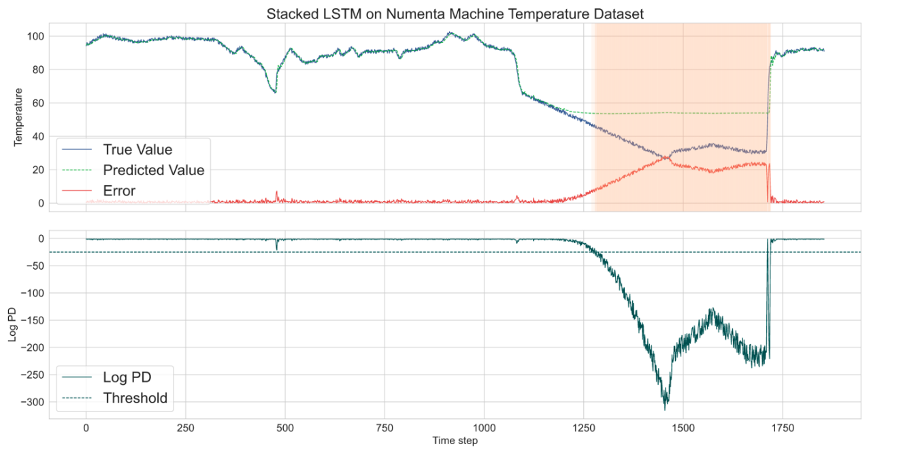
\includegraphics[scale=1.1]{./content/images/5-3.png}
    \caption{Phát hiện bất thường trên bộ dữ liệu nhiệt độ máy Numenta của mô hình đề xuất}
    \label{fig:5-3}
\end{figure}

Đối với giải thuật HOTSAX, chúng tôi tiến hành thiết lập các thông số như Bảng \ref{tab:5-1}, với bề rộng của sổ trượt \textit{n} là 128, hệ số thu giảm số chiều \textit{w} là 8 và số lượng các ký tự rời rạc hoá \textit{a} là 3. Bộ dữ liệu đã được tiền xử lý để có thể phù hợp với giải thuật HOTSAX từ các chuyên gia trong các công trình nghiên cứu trước đó.

\begin{figure}[H]
    \centering
    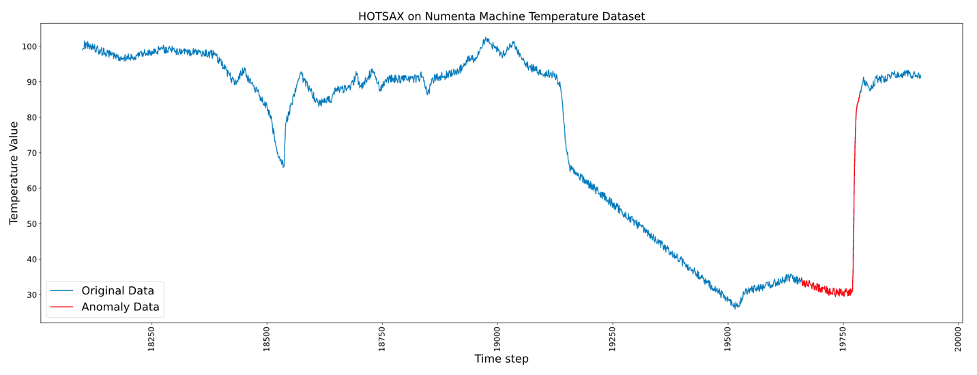
\includegraphics[scale=0.85]{./content/images/5-4.png}
    \caption{Phát hiện bất thường trên bộ dữ liệu nhiệt độ máy Numenta của HOTSAX}
    \label{fig:5-4}
\end{figure}

\begin{table}[H]
\centering
\begin{tabular}{|c|c|}
\hline
\textbf{Mô hình đề xuất} & \textbf{Giải thuật HOTSAX}  \\
\hline
4m6s                       & 39s                     \\
\hline
\end{tabular}
\caption{Thời gian thực thi trên bộ dữ liệu nhiệt độ máy Numenta}
\label{tab:5-2}
\end{table}

Kết quả phát hiện bất thường của mô hình đề xuất được thể hiện ở hình \ref{fig:5-3}, với biểu đồ bên trên thể hiện dữ liệu gốc, dữ liệu dự báo và sai số dự báo, vùng bóng mờ thể hiện bất thường được phát hiện. Biểu đồ bên dưới thể diện giá trị logPD và giá trị ngưỡng. Các điểm dữ liệu có giá trị logPD thấp hơn giá trị ngưỡng ở biểu đồ bên dưới, sẽ được phủ mờ tương ứng với biểu đồ bên trên. Kết quả phát hiện bất thường của giải thuật HOTSAX được thể hiện ở hình \ref{fig:5-4}. Ta có thể dễ dàng thấy được, cả hai giải thuật đều phát hiện được chuỗi con bất thường. Nhưng giải thuật HOTSAX chỉ phát hiện được nửa sau của chuỗi con bất thường. Trong khi ở mô hình đề xuất, chúng tôi đã phát hiện được chuỗi con bất thường sớm hơn, ngay khi giá trị nhiệt độ có xu hướng giảm liên tục trong một khoảng thời gian.

Xét về thời gian thực thi trong bảng \ref{tab:5-2}, chúng tôi nhận thấy mô hình đề xuất tốn nhiều thời gian hơn giải thuật HOTSAX. Điều này có thể được lý giải do mạng nơ-ron học sâu LSTM cần nhiều thời gian để huấn luyện trên bô dữ liệu này.

\subsection{Bộ dữ liệu power\_demand}
Mô hình LSTM xếp chồng được thiết lập với một tầng ẩn duy nhất với 300 nốt LSTM, theo sau là tầng kết nối đầy đủ với 1 nơ-ron đầu ra, hệ số học là 0.2. Và bộ thông số \textit{Adam optimizer}, \textit{learning-rate} là 0.01, \textit{decay} là 0.99, và 600 epoch có điều kiện dừng sớm. Từ mục 4.1.2, chúng tôi nhận thấy dữ liệu có chu kỳ thay đổi theo tuần, trong đó có năm ngày trong tuần sử dụng điện năng và hai ngày cuối tuần không sử dụng. Với \textit{batch-size} là 672, chúng tôi chia các \textit{batch} dữ liệu thành dữ liệu mỗi tuần. Kế tiếp, chúng tôi thực hiện duy trì trạng thái LSTM qua các \textit{batch}, bằng cách thiết lập \textit{stateful} bằng \textit{true}. Và với \textit{lookback} và \textit{lookahead} đều bằng 1, mô hình của chúng tôi đã có khả năng học được xu hướng dữ liệu. Giá trị MSE trên tập huấn luyện là 0.1019. Từ tập kiểm thử 2 $V_{A}$, với giá trị ngưỡng bằng -28, tất cả các điểm dữ liệu có giá trị logPD nhỏ hơn giá trị ngưỡng, chúng tôi xác định đó là các điểm bất thường, và ngược lại. Các điểm dữ liệu có giá trị logPD lớn hơn giá trị ngưỡng, chúng tôi xác định đó là các điểm bình thường. Với cách tiếp cận tương tự, chúng tôi dùng giá trị ngưỡng này cho tập kiểm tra \textit{T}.

\begin{figure}[H]
    \centering
    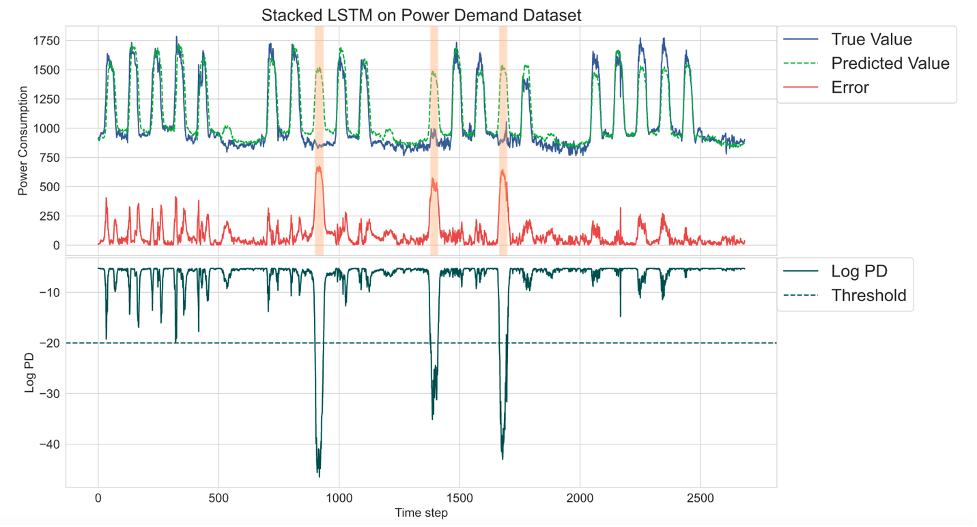
\includegraphics[scale=1]{./content/images/5-5.png}
    \caption{Phát hiện bất thường trên bộ dữ liệu power\_demand của mô hình đề xuất}
    \label{fig:5-5}
\end{figure}

Đối với giải thuật HOTSAX, chúng tôi tiến hành thiết lập các thông số như Bảng \ref{tab:5-1}, với bề rộng của sổ trượt \textit{n} là 1000. Chúng tôi kỳ vọng giải thuật sẽ nhận biết được sự khác nhau giữa tuần bình thường và tuần bất thường. Hệ số thu giảm số chiều \textit{w} là 8 và số lượng các ký tự rời rạc hoá \textit{a} là 3. Bộ dữ liệu đã được tiền xử lý để có thể phù hợp với giải thuật HOTSAX từ các chuyên gia trong các công trình nghiên cứu trước đó.

\begin{figure}[H]
    \centering
    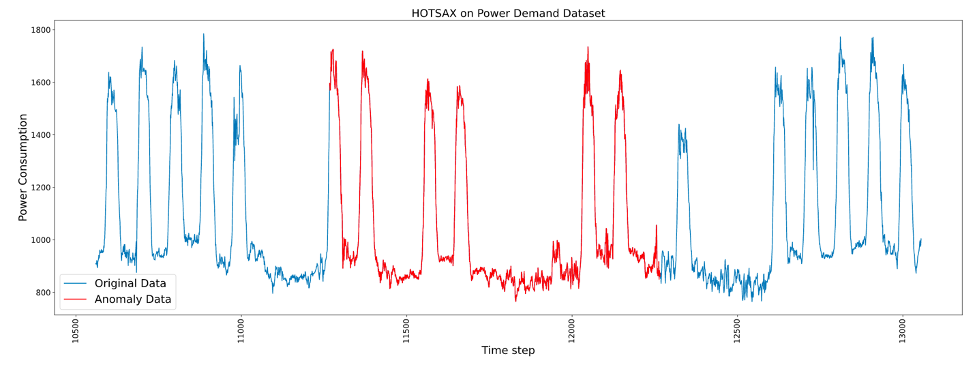
\includegraphics[scale=0.85]{./content/images/5-6.png}
    \caption{Phát hiện bất thường trên bộ dữ liệu power\_demand của HOTSAX}
    \label{fig:5-6}
\end{figure}

\begin{table}[H]
\centering
\begin{tabular}{|c|c|}
\hline
\textbf{Mô hình đề xuất} & \textbf{Giải thuật HOTSAX}  \\
\hline
13s                      & 5m18s                      \\
\hline
\end{tabular}
\caption{Thời gian thực thi trên bộ dữ liệu power\_demand}
\label{tab:5-3}
\end{table}

Kết quả phát hiện bất thường của mô hình đề xuất được thể hiện ở hình \ref{fig:5-5}, với biểu đồ bên trên thể hiện dữ liệu gốc, dữ liệu dự báo và sai số dự báo, vùng bóng mờ thể hiện bất thường được phát hiện. Biểu đồ bên dưới thể diện giá trị logPD và giá trị ngưỡng. Các điểm dữ liệu có giá trị logPD thấp hơn giá trị ngưỡng ở biểu đồ bên dưới, sẽ được phủ mờ tương ứng với biểu đồ bên trên. Kết quả phát hiện bất thường của giải thuật HOTSAX được thể hiện ở hình \ref{fig:5-6}. Dễ dàng nhận thấy, cả hai đều phát hiện được chuỗi con bất thường. Đó là hai tuần có ngày lễ. Tuần thứ nhất có ngày lễ \textit{Queen’s Birthday} vào thứ tư và tuần thứ hai có hai ngày lễ là ngày \textit{Liberation Day} và \textit{Ascension Day} vào thứ hai và thứ năm. Trong các ngày lễ này, không có tiêu thụ điện năng tại trung tâm nghiên cứu, nên dữ liệu tại những ngày này sẽ không có gai nhọn. Đi sâu vào chuỗi con bất thường, chúng tôi nhận thấy giải thuật HOTSAX có các cảnh báo sai tại những ngày có tiêu thụ điện năng. Nguyên nhân là do kích thước cửa sổ trượt, chúng tôi đã thử những kích thước cửa sổ khác nhau. Nhưng đây là kích thước cho kết quả ổn định nhất. Lúc này mô hình đề xuất đã phát huy được ưu thế do không dựa vào kích thước cửa sổ trượt, chúng tôi đã cảnh báo được các ngày bất thường trong hai tuần có dữ liệu bất thường và không có cảnh báo sai đối với ba ngày còn lại. 

Xét về thời gian thực thi trong bảng \ref{tab:5-3}, mô hình đề xuất có thời gian thực thi ngắn hơn rất nhiều so với giải thuật HOTSAX. Điều này chúng tỏ, mô hình đề xuất của chúng tôi đã học được chu kỳ dữ liệu và quá trình huấn luyện được dừng sớm khi giá trị hàm mất mát không giảm qua các epoch. Đối với giải thuật HOTSAX, kích thước cửa sổ trượt và kích thước của bộ dữ liệu là nguyên nhân của việc tốn nhiều thời gian thực thi. Do chúng tôi chọn kích thước cửa sổ là 1000, nên giải thuật cần rất nhiều thời gian để mã hóa ký tự SAX. Với kích thước bộ dữ liệu là 35040, giải thuật HOTSAX cũng cần nhiều thời gian để quét hết bộ dữ liệu.

\subsection{Bộ dữ liệu TEK16}
Mô hình LSTM xếp chồng được thiết lập với hai tầng ẩn, với 80 nốt LSTM cho tầng ẩn đầu tiên và 30 nốt LSTM cho tầng ẩn thứ hai, theo sau là tầng kết nối đầy đủ với 1 nơ-ron đầu ra, hệ số học là 0.2. Và bộ thông số \textit{Adam optimizer}, \textit{learning-rate} là 0.01, \textit{decay} là 0.99, và 600 epoch có điều kiện dừng sớm. Từ mục 4.1.4, chúng tôi nhận thấy dữ liệu có chu kỳ thay đổi theo từng chu kỳ năng lượng.Với \textit{batch-size} là 1000, chúng tôi chia các \textit{batch} dữ liệu thành dữ liệu mỗi chu kỳ năng lượng đi qua van. Kế tiếp, chúng tôi thực hiện duy trì trạng thái LSTM qua các \textit{batch}, bằng cách thiết lập \textit{stateful} bằng \textit{true}. Với \textit{lookback} và \textit{lookahead} đều bằng 1, mô hình của chúng tôi đã có khả năng học được xu hướng dữ liệu. Giá trị MSE trên tập huấn luyện là 0.1401. Từ tập kiểm thử 2 $V_{A}$, với giá trị ngưỡng bằng -20, tất cả các điểm dữ liệu có giá trị logPD nhỏ hơn giá trị ngưỡng, chúng tôi xác định đó là các điểm bất thường, và ngược lại. Các điểm dữ liệu có giá trị logPD lớn hơn giá trị ngưỡng, chúng tôi xác định đó là các điểm bình thường. Với cách tiếp cận tương tự, chúng tôi dùng giá trị ngưỡng này cho tập kiểm tra \textit{T}.

\begin{figure}[H]
    \centering
    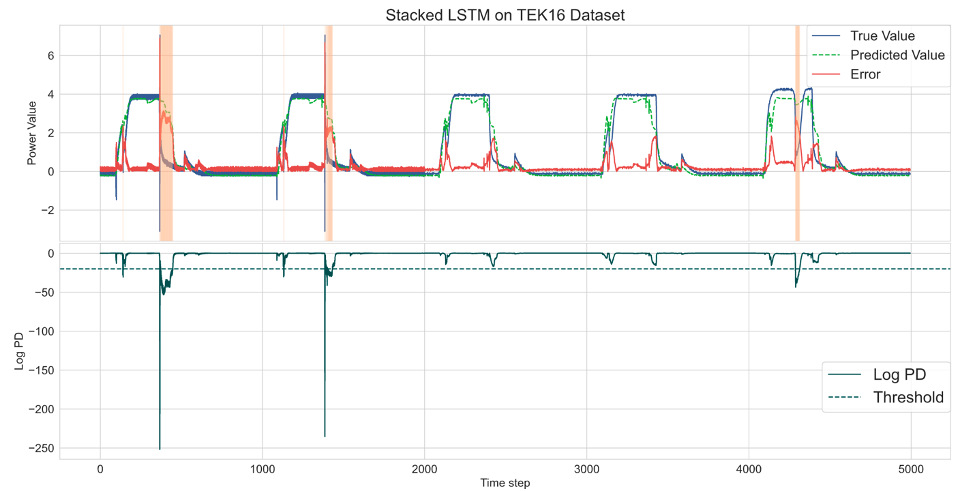
\includegraphics[scale=1]{./content/images/5-9.png}
    \caption{Phát hiện bất thường trên bộ dữ liệu TEK16 của mô hình đề xuất}
    \label{fig:5-9}
\end{figure}

Đối với giải thuật HOTSAX, vẫn như các bộ dữ liệu khác, chúng tôi tiến hành thiết lập các thông số như Bảng \ref{tab:5-1}, với bề rộng của sổ trượt \textit{n} là 128, hệ số thu giảm số chiều \textit{w} là 8 và số lượng các ký tự rời rạc hoá \textit{a} là 3. Bộ dữ liệu đã được tiền xử lý để có thể phù hợp với giải thuật HOTSAX từ các chuyên gia trong các công trình nghiên cứu trước đó.

\begin{figure}[H]
    \centering
    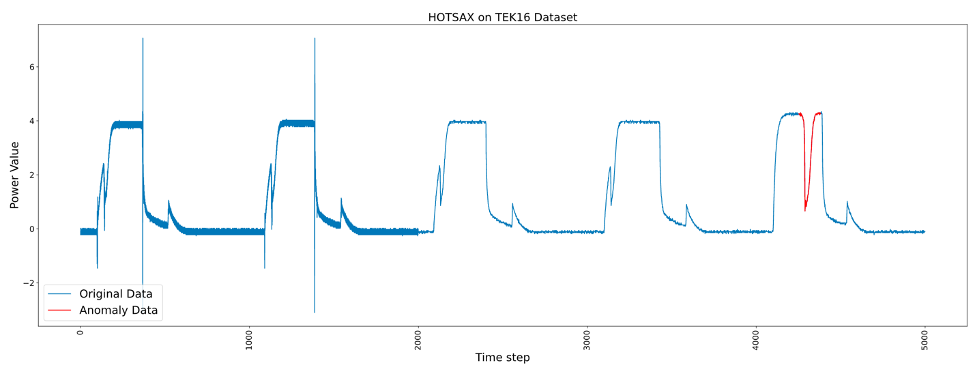
\includegraphics[scale=0.75]{./content/images/5-10.png}
    \caption{Phát hiện bất thường trên bộ dữ liệu TEK16 của HOTSAX}
    \label{fig:5-10}
\end{figure}

\begin{table}[H]
\centering
\begin{tabular}{|c|c|}
\hline
\textbf{Mô hình đề xuất} & \textbf{Giải thuật HOTSAX}  \\
\hline
9s                       & 7s                     \\
\hline
\end{tabular}
\caption{Thời gian thực thi trên bộ dữ liệu TEK16}
\label{tab:5-5}
\end{table}

Kết quả phát hiện bất thường của mô hình đề xuất được thể hiện ở hình \ref{fig:5-9}, với biểu đồ bên trên thể hiện dữ liệu gốc, dữ liệu dự báo và sai số dự báo, vùng bóng mờ thể hiện bất thường được phát hiện. Biểu đồ bên dưới thể diện giá trị logPD và giá trị ngưỡng. Các điểm dữ liệu có giá trị logPD thấp hơn giá trị ngưỡng ở biểu đồ bên dưới, sẽ được phủ mờ tương ứng với biểu đồ bên trên. Kết quả phát hiện bất thường của giải thuật HOTSAX được thể hiện ở hình \ref{fig:5-10}. Dễ dàng nhận thấy, giải thuật HOTSAX đã phát hiện bất thường rất tốt ở bộ dữ liệu này. Mô hình đề xuất cũng phát hiện được chuỗi con bất thường ở bộ dữ liệu này. Nhưng bên cạnh đó, mô hình đề xuất cũng có hai cảnh báo sai tại hai chu kỳ năng lượng đầu tiên của bộ dữ liệu. Một điều nữa, sai số dự báo của mô hình đề xuất cũng khá cao, đặc biệt trong những lúc thay đổi giá trị trong một chu kỳ năng lượng. Một điều dễ dàng nhận thấy là chúng tôi thiếu dữ liệu huấn luyện cho bộ dữ liệu này. Trong năm chu kỳ dữ liệu, chỉ có chu kỳ thứ ba và chu kỳ thứ tư dùng được cho tập huấn luyện, điều này dẫn tới mô hình đề xuất học không tốt xu hướng của dữ liệu. Đây cũng là nhược điểm của mô hình đề xuất nói riêng, và cũng là nhược điểm của các mô hình dự báo nói chung.

Xét về thời gian thực thi trong bảng \ref{tab:5-5}, có sự khác biệt không quá lớn giữa mô hình đề xuất và giải thuật HOTSAX. Xem xét xu hướng dữ liệu, chúng tôi nhận thấy bộ dữ liệu có chứa các chu kỳ của dữ liệu. Điều này làm mô hình đề xuất của chúng tôi đã học được chu kỳ của dữ liệu rất sớm, nên tổng thời gian phát hiện bất thường giảm. Đối với giải thuật HOTSAX, với kích thước cửa sổ trượt là 128, và sự khác biệt lớn giữa chuỗi con bất thường so với các chuỗi con còn lại giúp chúng tôi tìm ra chuỗi con bất thường với thời gian thực thi ngắn.

\subsection{Bộ dữ liệu chứng khoán stock\_20\_0}
Mô hình LSTM xếp chồng được thiết lập với \textit{lookback} là 5, \textit{lookahead} là 3, với hai tầng ẩn lần lượt 60 nốt LSTM và 30 nốt LSTM, theo sau là tầng kết nối đầy đủ với 1 nơ-ron đầu ra, hệ số học là 0.1. Chúng tôi huấn luyện mô hình với bộ thông số \textit{Adam optimizer}, \textit{learning-rate} là 0.1, \textit{decay} là 0.99, và 600 epoch có điều kiện dừng sớm, \textit{batch-size} là 256. Vì bộ dữ liệu không chứa bất kỳ mẫu lặp lại nào nên chúng tôi đã không duy trì trạng thái LSTM giữa các \textit{batch}, tức \textit{stateful} bằng \textit{false}. Giá trị MSE trên tập huấn luyện là 0.0242. Từ tập kiểm thử 2 $V_{A}$, với giá trị ngưỡng bằng -5, tất cả các điểm dữ liệu có giá trị logPD nhỏ hơn giá trị ngưỡng, chúng tôi xác định đó là các điểm bất thường, và ngược lại. Các điểm dữ liệu có giá trị logPD lớn hơn giá trị ngưỡng, chúng tôi xác định đó là các điểm bình thường. Với cách tiếp cận tương tự, chúng tôi dùng giá trị ngưỡng này cho tập kiểm tra \textit{T}.

\begin{figure}[H]
    \centering
    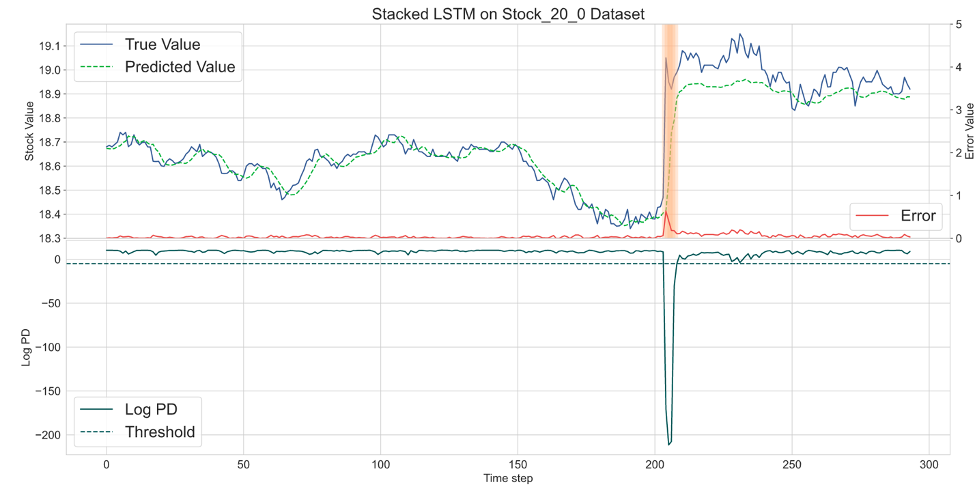
\includegraphics[scale=1]{./content/images/5-11.png}
    \caption{Phát hiện bất thường trên bộ dữ liệu stock\_20\_0 của mô hình đề xuất}
    \label{fig:5-11}
\end{figure}

Vẫn như các bộ dữ liệu khác, đối với giải thuật HOTSAX, chúng tôi tiến hành thiết lập các thông số như Bảng \ref{tab:5-1}, với bề rộng của sổ trượt \textit{n} là 128, hệ số thu giảm số chiều \textit{w} là 8 và số lượng các ký tự rời rạc hoá \textit{a} là 3. Bộ dữ liệu đã được tiền xử lý để có thể phù hợp với giải thuật HOTSAX từ các chuyên gia trong các công trình nghiên cứu trước đó.

\begin{figure}[H]
    \centering
    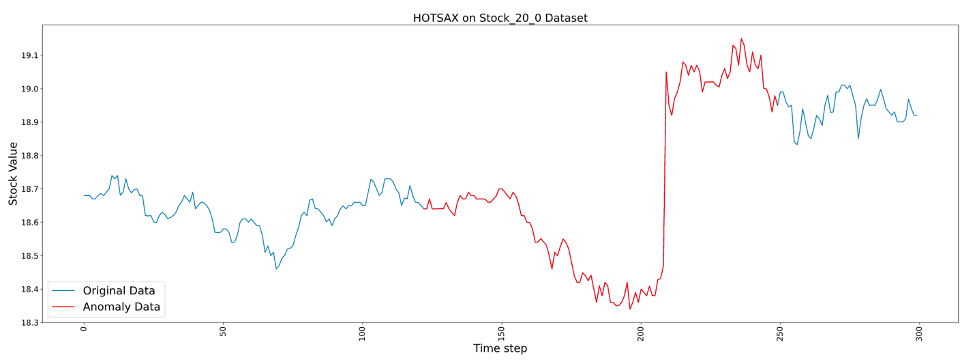
\includegraphics[scale=0.75]{./content/images/5-12.png}
    \caption{Phát hiện bất thường trên bộ dữ liệu stock\_20\_0 của HOTSAX}
    \label{fig:5-12}
\end{figure}

\begin{table}[H]
\centering
\begin{tabular}{|c|c|}
\hline
\textbf{Mô hình đề xuất} & \textbf{Giải thuật HOTSAX}  \\
\hline
34s                       & 9s                     \\
\hline
\end{tabular}
\caption{Thời gian thực thi trên bộ dữ liệu stock\_20\_0}
\label{tab:5-6}
\end{table}

Kết quả phát hiện bất thường của mô hình đề xuất được thể hiện ở hình \ref{fig:5-11}, với biểu đồ bên trên thể hiện dữ liệu gốc, dữ liệu dự báo và sai số dự báo, vùng bóng mờ thể hiện bất thường được phát hiện. Biểu đồ bên dưới thể diện giá trị logPD và giá trị ngưỡng. Các điểm dữ liệu có giá trị logPD thấp hơn giá trị ngưỡng ở biểu đồ bên dưới, sẽ được phủ mờ tương ứng với biểu đồ bên trên. Kết quả phát hiện bất thường của giải thuật HOTSAX được thể hiện ở hình \ref{fig:5-12}. Cả hai phương pháp đều phát hiện được chuỗi con bất thường. Đi sâu vào chuỗi con bất thường, chúng tôi nhận thấy giải thuật HOTSAX đã có những cảnh báo sai trước khi giá trị cổ phiếu tăng một cách đột ngột. Nhưng ở mô hình đề xuất, chúng tôi đã phát hiện bất thường ngay lúc giá trị tăng đột ngột và không có cảnh báo sai. Nguyên nhân của điều này là do giải thuật HOTSAX dựa vào kích thước cửa sổ trượt, còn mô hình đề xuất thì không. Đây có thể xem như ưu thế của mô hình đề xuất nói riêng và phương pháp phát hiện bất thường bằng dự báo nói chung.

Xét về thời gian thực thi trong bảng \ref{tab:5-6}, chúng tôi nhận thấy mô hình đề xuất cần nhiều thời gian để thực thi hơn giải thuật HOTSAX. Cũng như các bộ dữ liệu khác, mô hình đề xuất của chúng tôi cần nhiều thời gian để huấn luyện, dẫn tới tổng thời gian phát hiện bất thường tăng lên.

\subsection{Bộ dữ liệu memory}
Mô hình LSTM xếp chồng được thiết lập với \textit{lookback} là 5, \textit{lookahead} là 3, với hai tầng ẩn lần lượt 60 nốt LSTM và 30 nốt LSTM, theo sau là tầng kết nối đầy đủ với 1 nơ-ron đầu ra, hệ số học là 0.1. Chúng tôi huấn luyện mô hình với bộ thông số \textit{Adam optimizer}, \textit{learning-rate} là 0.1, decay là 0.99, và 600 epoch có điều kiện dừng sớm, \textit{batch-size} là 256. Vì bộ dữ liệu không chứa bất kỳ mẫu lặp lại nào nên chúng tôi đã không duy trì trạng thái LSTM giữa các \textit{batch}, tức \textit{stateful} bằng \textit{false}. Giá trị MSE trên tập huấn luyện là 0.0209. Từ tập kiểm thử 2 $V_{A}$, với giá trị ngưỡng bằng -13, tất cả các điểm dữ liệu có giá trị logPD nhỏ hơn giá trị ngưỡng, chúng tôi xác định đó là các điểm bất thường, và ngược lại. Các điểm dữ liệu có giá trị logPD lớn hơn giá trị ngưỡng, chúng tôi xác định đó là các điểm bình thường. Với cách tiếp cận tương tự, chúng tôi dùng giá trị ngưỡng này cho tập kiểm tra \textit{T}.

\begin{figure}[H]
    \centering
    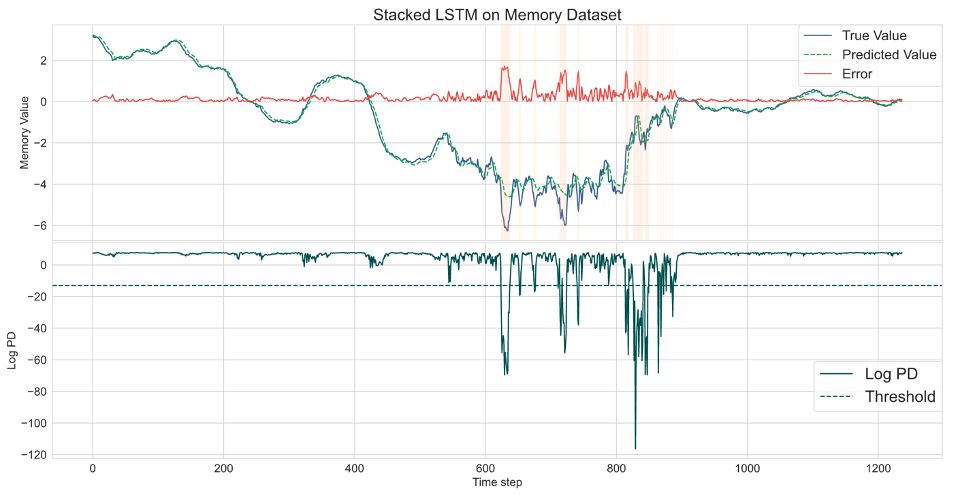
\includegraphics[scale=1]{./content/images/5-13.png}
    \caption{Phát hiện bất thường trên bộ dữ liệu memory của mô hình đề xuất}
    \label{fig:5-13}
\end{figure}

Đối với giải thuật HOTSAX, chúng tôi tiến hành thiết lập các thông số như Bảng \ref{tab:5-1}, với bề rộng của sổ trượt \textit{n} là 128, hệ số thu giảm số chiều \textit{w} là 8 và số lượng các ký tự rời rạc hoá \textit{a} là 3. Bộ dữ liệu đã được tiền xử lý để có thể phù hợp với giải thuật HOTSAX từ các chuyên gia trong các công trình nghiên cứu trước đó.

\begin{figure}[H]
    \centering
    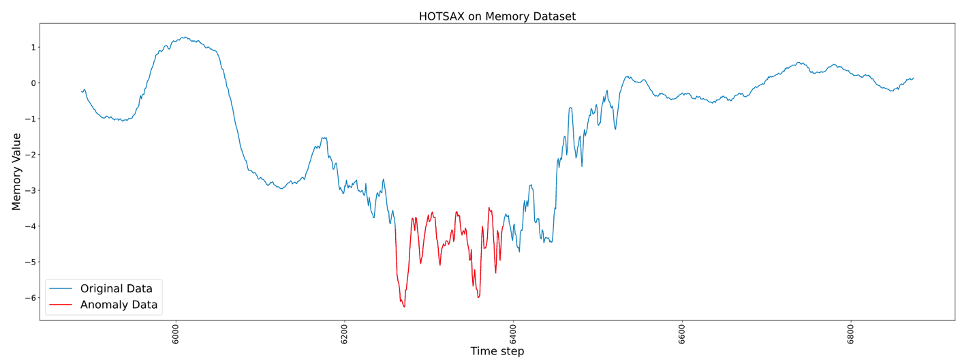
\includegraphics[scale=0.75]{./content/images/5-14.png}
    \caption{Phát hiện bất thường trên bộ dữ liệu memory của HOTSAX}
    \label{fig:5-14}
\end{figure}

\begin{table}[H]
\centering
\begin{tabular}{|c|c|}
\hline
\textbf{Mô hình đề xuất} & \textbf{Giải thuật HOTSAX}  \\
\hline
27s                       & 11s                     \\
\hline
\end{tabular}
\caption{Thời gian thực thi trên bộ dữ liệu memory}
\label{tab:5-7}
\end{table}

Kết quả phát hiện bất thường của mô hình đề xuất được thể hiện ở hình \ref{fig:5-13}, với biểu đồ bên trên thể hiện dữ liệu gốc, dữ liệu dự báo và sai số dự báo, vùng bóng mờ thể hiện bất thường được phát hiện. Biểu đồ bên dưới thể diện giá trị logPD và giá trị ngưỡng. Các điểm dữ liệu có giá trị logPD thấp hơn giá trị ngưỡng ở biểu đồ bên dưới, sẽ được phủ mờ tương ứng với biểu đồ bên trên. Kết quả phát hiện bất thường của giải thuật HOTSAX được thể hiện ở hình \ref{fig:5-14}. Nhìn chung cả hai phương pháp đều phát hiện được chuỗi con bất thường. Nhưng ở giải thuật HOTSAX, chúng tôi không thể phát hiện hết chuỗi con bất thường do giới hạn của cửa sổ trượt. Chúng tôi cũng đã thử các kích thước cửa sổ trượt lớn hơn, nhưng kết quả không được tốt bằng kích thước hiện tại. Đối với mô hình đề xuất, chúng tôi đã phát hiện được hầu hết bất thường của chuỗi con bất thường.

Xét về thời gian thực thi trong bảng \ref{tab:5-7}, cũng giống như bộ dữ liệu stock\_20\_0, chúng tôi nhận thấy mô hình đề xuất cần nhiều thời gian để thực thi hơn giải thuật HOTSAX. Như đã đề cập trong các bộ dữ liệu khác, mô hình đề xuất của chúng tôi cần nhiều thời gian để huấn luyện, dẫn tới tổng thời gian phát hiện bất thường tăng lên.

\subsection{Bộ dữ liệu ann\_gun\_CentroidA}
Đây là bộ dữ liệu 2D, chứa hai chuỗi thời gian đo toạ độ X và Y của tay diễn viên, nên bộ dữ liệu này có hai kênh X và Y tương ứng với hai bộ dữ liệu nhỏ. Chúng tôi quyết định phát hiện bất thường lần lượt trên cả hai kênh này, bằng cách tách thành hai bộ dữ liệu nhỏ, tương ứng với từng kênh và lần lượt huấn luyện và phát hiện bất thường trên cùng một mô hình.

Mô hình LSTM xếp chồng được thiết lập cho cả hai kênh với hai tầng ẩn, với 80 nốt LSTM cho tầng ẩn đầu tiên và 30 nốt LSTM cho tầng ẩn thứ hai, theo sau là tầng kết nối đầy đủ với 1 nơ-ron đầu ra, hệ số học là 0.2. Và bộ thông số \textit{Adam optimizer}, \textit{learning-rate} là 0.01, \textit{decay} là 0.99, và 600 epoch có điều kiện dừng sớm. Chúng tôi nhận thấy bộ dữ liệu có các gợn sóng theo chu kỳ cho cả hai kênh. Với \textit{batch-size} bằng 150, chúng tôi chia các gợn sóng vào các \textit{batch} dữ liệu. Kế tiếp, chúng tôi thực hiện duy trì trạng thái LSTM qua các \textit{batch}, bằng cách thiệt lập \textit{stateful} bằng \textit{true}. Với \textit{lookback} và \textit{lookahead} đều bằng 1, mô hình của chúng tôi đã có khả năng học được xu hướng dữ liệu. Giá trị MSE trên tập huấn luyện trên kênh X và kênh Y lần lượt là là 0.1245 và 0.0962. Từ tập kiểm thử 2 $V_{A}$ của bộ dữ liệu từng kênh,chúng tôi xác định giá trị ngưỡng cho kênh X và kênh Y lần lượt là -8 và -9. Trên tập dữ liệu của từng kênh, tất cả các điểm dữ liệu có giá trị logPD nhỏ hơn giá trị ngưỡng, chúng tôi xác định đó là các điểm bất thường, và ngược lại. Các điểm dữ liệu có giá trị logPD lớn hơn giá trị ngưỡng, chúng tôi xác định đó là các điểm bình thường. Với cách tiếp cận tương tự, chúng tôi dùng giá trị ngưỡng này cho tập kiểm tra \textit{T} cho từng kênh.

\begin{figure}[H]
    \centering
    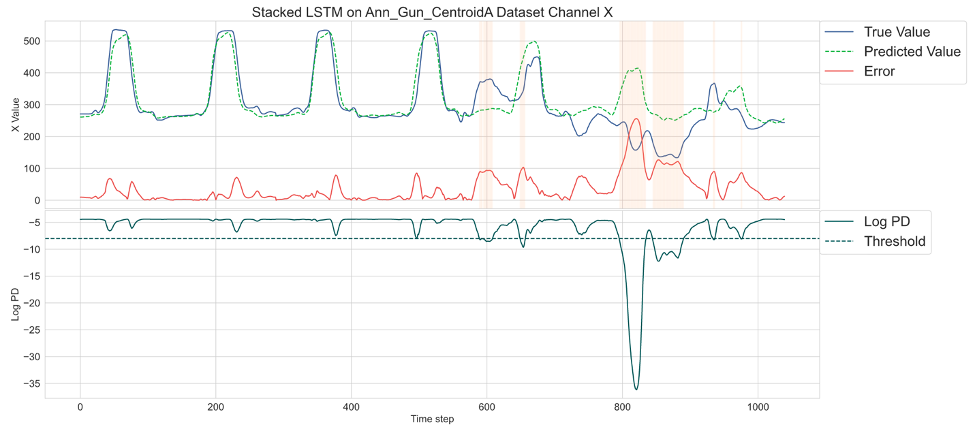
\includegraphics[scale=1]{./content/images/5-15.png}
    \caption{Phát hiện bất thường trên bộ dữ liệu ann\_gun\_CentroidA kênh X của mô hình đề xuất}
    \label{fig:5-15}
\end{figure}

\begin{figure}[H]
    \centering
    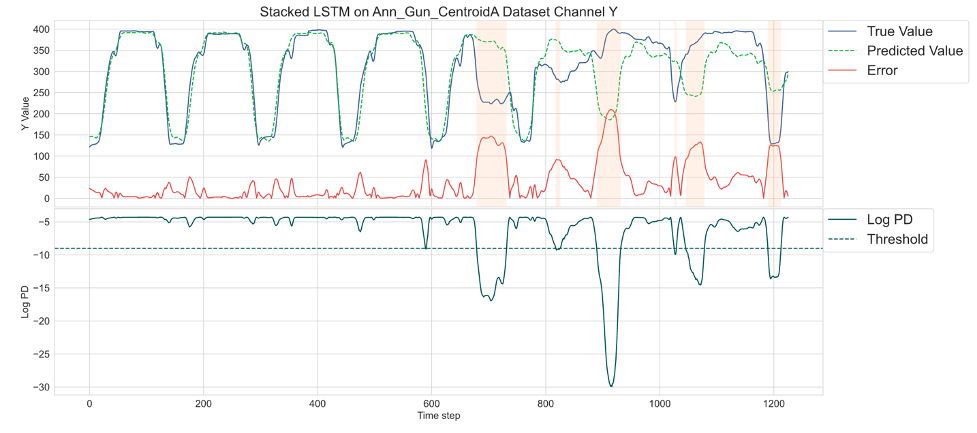
\includegraphics[scale=1]{./content/images/5-16.png}
    \caption{Phát hiện bất thường trên bộ dữ liệu ann\_gun\_CentroidA kênh Y của mô hình đề xuất}
    \label{fig:5-16}
\end{figure}

Cũng tương tự như mô hình đề xuất, chúng tôi cũng chia bộ dữ liệu gốc thành hai bộ dữ liệu nhỏ tương ứng với bộ dữ liệu của từng kênh và thực hiện giải thuật HOTSAX trên từng bộ dữ liệu này. Chúng tôi tiến hành thiết lập các thông số như Bảng \ref{tab:5-1}, với bề rộng của sổ trượt \textit{n} là 128, hệ số thu giảm số chiều \textit{w} là 8 và số lượng các ký tự rời rạc hoá \textit{a} là 3. Giải thuật HOTSAX chạy trên từng bộ dữ liệu của từng kênh và đã được tiền xử lý để có thể phù hợp với giải thuật HOTSAX từ các chuyên gia trong các công trình nghiên cứu trước đó.

\begin{figure}[H]
    \centering
    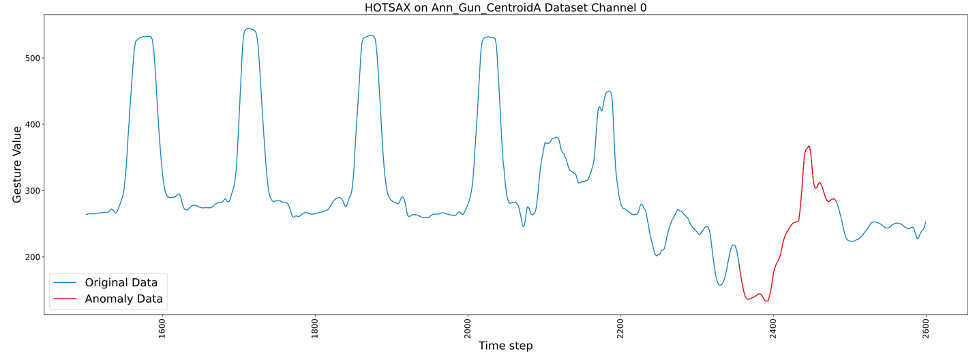
\includegraphics[scale=0.75]{./content/images/5-17.png}
    \caption{Phát hiện bất thường trên bộ dữ liệu ann\_gun\_CentroidA kênh X của HOTSAX}
    \label{fig:5-17}
\end{figure}

\begin{figure}[H]
    \centering
    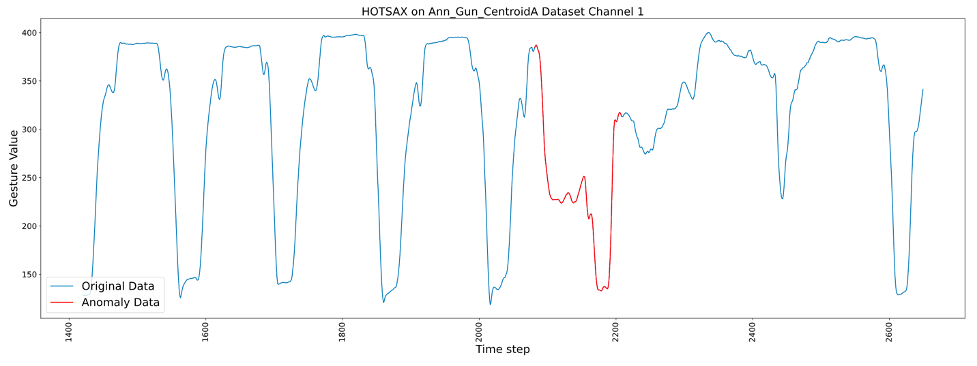
\includegraphics[scale=0.75]{./content/images/5-18.png}
    \caption{Phát hiện bất thường trên bộ dữ liệu ann\_gun\_CentroidA kênh Y của HOTSAX}
    \label{fig:5-18}
\end{figure}

\begin{table}[H]
\centering
\begin{tabular}{|c|c|c|}
\hline
\textbf { } & \textbf{Mô hình đề xuất} & \textbf{Giải thuật HOTSAX}  \\
\hline
\textbf { Kênh X } & 1m7s                       & 17s                     \\
\hline
\textbf { Kênh Y } & 51s                       & 15s                     \\
\hline
\end{tabular}
\caption{Thời gian thực thi trên bộ dữ liệu ann\_gun\_CentroidA}
\label{tab:5-8}
\end{table}

Kết quả phát hiện bất thường của mô hình đề xuất được thể hiện ở hình \ref{fig:5-15} và hình \ref{fig:5-16}, với biểu đồ bên trên thể hiện dữ liệu gốc, dữ liệu dự báo và sai số dự báo, vùng bóng mờ thể hiện bất thường được phát hiện. Biểu đồ bên dưới thể diện giá trị logPD và giá trị ngưỡng. Các điểm dữ liệu có giá trị logPD thấp hơn giá trị ngưỡng ở biểu đồ bên dưới, sẽ được phủ mờ tương ứng với biểu đồ bên trên. Kết quả phát hiện bất thường của giải thuật HOTSAX được thể hiện ở hình \ref{fig:5-17} và hình \ref{fig:5-18}. 

Đối với bộ dữ liệu của kênh X, cả hai phương pháp đều phát hiện được chuỗi con bất thường. Nhưng mô hình đề xuất đã phát hiện được ngay khi bắt đầu có sự bất thường và hầu hết các phần còn lại của chuỗi con bất thường. Đối với giải thuật HOTSAX, do hạn chế về kích thước cửa sổ trượt, nên giải thuật chỉ phát hiện được một phần của chuỗi con bất thường. Mặc dù chúng tôi đã thử những kích thước cửa sổ trượt lớn hơn, nhưng đây là kết quả ổn định nhất.

Đối với bộ dữ liệu của kênh Y, chúng tôi nhận thấy cả hai phương pháp đều phát hiện được ngay khi có bắt đầu có sự bất thường. Do hạn chế về kích thước của sổ trượt, nên giải thuật HOTSAX chỉ phát hiện được phần đầu của chuỗi con bất thường. Nhờ vào không có sự phụ thuộc vào kích thước cửa sổ trượt, nên mô hình đề xuất đã phát hiện được hầu hết phần còn lại của chuỗi con bất thường.

Xét về thời gian thực thi trong bảng \ref{tab:5-8}, mô hình đề xuất của chúng tôi cần nhiều thời gian thực thi hơn giải thuật HOTSAX trên cả hai bộ dữ liệu. Điều này chứng tỏ mô hình đề xuất cần nhiều thời gian để huấn luyện trên các bộ dữ liệu này. Một điều khác, mô hình đề xuất cần nhiều thời gian để huấn luyện trên bộ dữ liệu kênh X, nên thời gian thực thi trên bộ dữ liệu X lớn hơn thời gian thực thi trên bộ dữ liệu Y. 

\section{Kết luận}
Nhìn chung, giải thuật HOTSAX và mô hình đề xuất đều phát hiện được những chuỗi con bất thường trên từng bộ dữ liệu. Với ưu thế dựa vào dự báo và phát hiện bất thường bằng sai số dự báo, mô hình đề xuất đã phát hiện được những điểm bất thường nhất của chuỗi con bất thường, đồng thời cũng tránh được những hạn chế của việc dựa vào kích thước cửa sổ trượt. Nhưng điều này cũng gây ra những cảnh báo sai, khi sai số dự báo quá lớn. Đặc biệt là đối với các bộ dữ liệu có ít dữ liệu huấn luyện. Đối với giải thuật HOTSAX, nhờ những ưu thế nhất định khi dựa vào kích thước cửa sổ trượt, giải thuật hoạt động ổn định trên các bộ dữ liệu, và không có cảnh báo sai ngoài chuỗi con bất thường.

Trong giải thuật HOTSAX, các chuỗi con được xác định bằng cửa sổ trượt. Bằng cách tính toán khoảng cách giữa các chuỗi con để tìm ra chuỗi con bất thường nhất. Điều này sẽ gặp vấn đề khi bộ dữ liệu chứa hai hay nhiều chuỗi con bất thường giống nhau, khi đó kết quả phát hiện bất thường sẽ không còn được chính xác. Đối với mô hình đề xuất, vấn đề này đã được khắc phục nhờ vào phương pháp phát hiện bất thường dựa vào dự báo. Sai số dự báo được dùng để xác định chuỗi con bất thường. Do đó, cho dù bộ dữ liệu chứa hai hay nhiều chuỗi con bất thường giống nhau, mô hình đề xuất vẫn sẽ phát hiện ra được. Chúng tôi đã thực nghiệm điều này bằng cách nhân bản bộ dữ liệu ECG lên 2 lần và thực hiện phát hiện bất thường trên bộ dữ liệu mới này bằng giải thuật HOTSAX và mô hình đề xuất.

\begin{figure}[H]
    \centering
    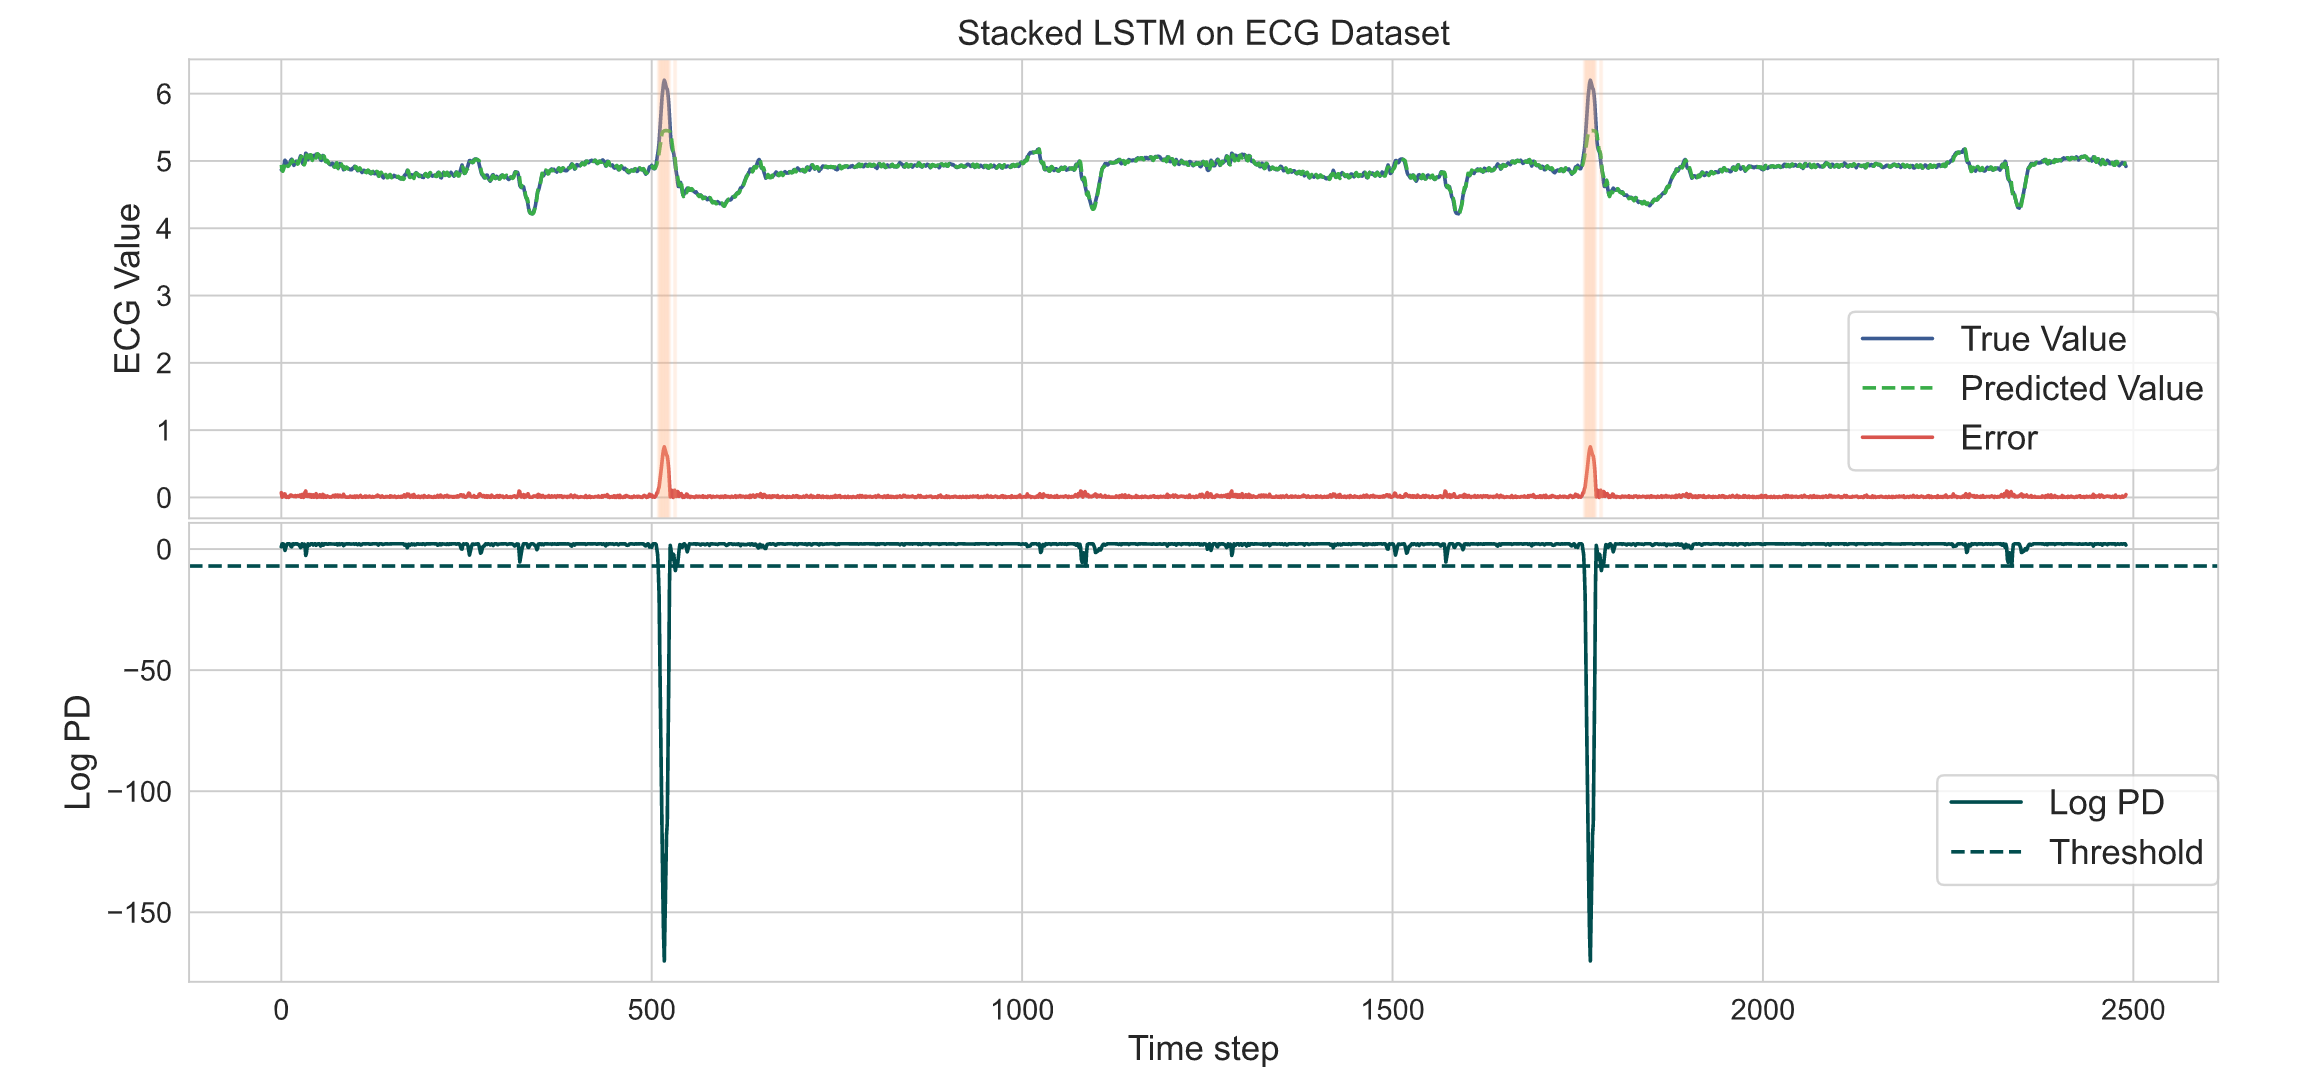
\includegraphics[scale=0.4]{./content/images/5-19.png}
    \caption{Phát hiện bất thường trên bộ dữ liệu ECG nhân bản của mô hình đề xuất}
    \label{fig:5-19}
\end{figure}

\begin{figure}[H]
    \centering
    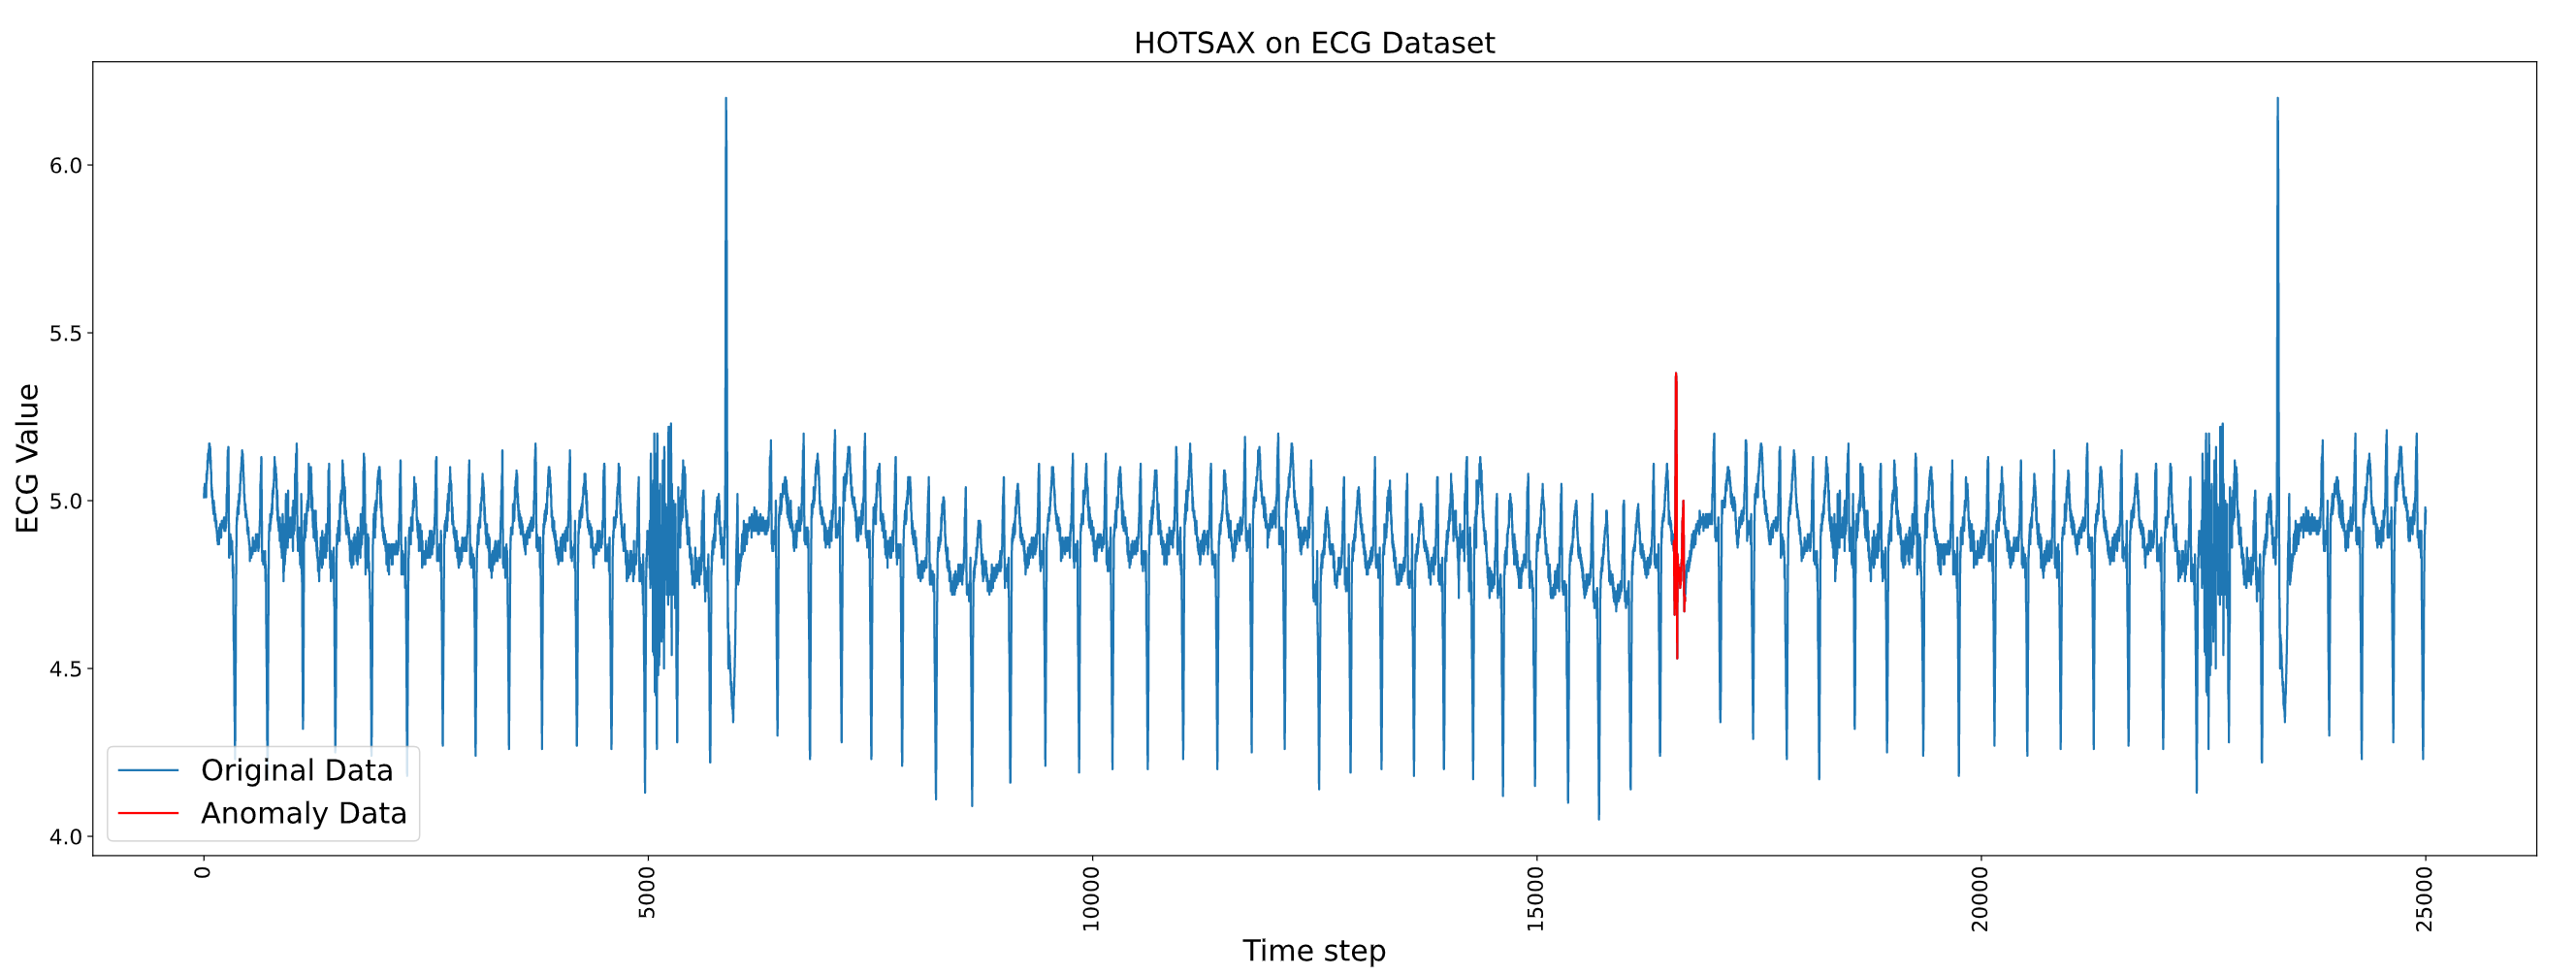
\includegraphics[scale=0.35]{./content/images/5-20.png}
    \caption{Phát hiện bất thường trên bộ dữ liệu ECG nhân bản của HOTSAX}
    \label{fig:5-20}
\end{figure}

Kết quả phát hiện bất thường của mô hình đề xuất được thể hiện ở hình \ref{fig:5-19} và kết quả của giải thuật HOTSAX ở hình \ref{fig:5-20}. Dễ dàng nhận thấy, giải thuật HOTSAX đã phát hiện sai chuỗi con bất thường khi có 2 phiên bản giống nhau của chuỗi con bất thường nhất. Đây chính là nhược điểm trong cách tiếp cận dựa vào kích thước của sổ trượt và khoảng cách giữa các chuỗi con mà chúng tôi đã đề cập ở trên. Khác với giải thuật HOTSAX, mô hình đề xuất vẫn phát hiện được 2 chuỗi con bất thường dựa vào sai số dự báo. Vì mô hình đề xuất đã học được xu hướng của dữ liệu, cho nên nếu có thêm 1 phiên bản chuỗi con bất thường, mô hình vẫn có thể phát hiện nhờ sai số dự báo tại các điểm bất thường. Điều này có ý nghĩa rất quan trọng trong thực tế, khi mà dữ liệu luôn có nhiều hơn 1 chuỗi con bất thường.

Xét về thời gian thực thi, khó có thể đưa ra sự so sánh chính xác về thời gian thực thi của mô hình đề xuất và giải thuật HOTSAX, do mỗi phương pháp có một cách thức hoạt động khác nhau. Với mô hình đề xuất, thời gian thực thi phụ thuộc vào thời gian gian huấn luyện mô hình. Quá trình này phụ thuộc vào nhiều yếu tố như độ lớn của tập dữ liệu, kích thước đầu vào, độ phức tạp của mô hình...Đối với giải thuật HOTSAX, thời gian thực thi sẽ phụ thuộc phần lớn vào kích thước cửa sổ trượt, và kích thước bộ dữ liệu. Qua kết quả thu được về thời gian thực thi của hai phương pháp, phần lớn giải thuật HOTSAX có thời gian thực thi nhỏ hơn mô hình đề xuất. Chỉ có bộ dữ liệu power\_demand với kích thước bộ dữ liệu và cửa sổ trượt lớn, giải thuật HOTSAX có thời gian thực thi lớn hơn giải thuật đề xuất. Với sự phát triển về phần cứng và giải thuật, chúng tôi tin rằng thời gian huấn luyện mô hình của các mạng nơ-ron học sâu sẽ được cải thiện, và phương pháp phát hiện bất thường bằng dự báo sẽ được cải thiện trong tương lai.

